\subsection{A smoothing function}
\label{sec:argumentforepsilon}
\begin{wrapfigure}{r}{0.4\textwidth}
\begin{center}
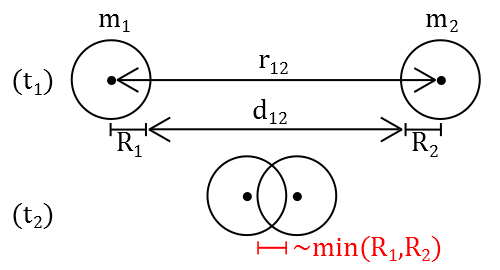
\includegraphics[width = 0.4\textwidth]{Figures/argument_for_epsilon.png}
\end{center}
\caption{Stars in motion}
\label{fig:afeps}
\end{wrapfigure}

Simulating two stars moving around each other in space, the method used is looking at them as point particles. This method is good to some extent, but it allows the stars to pass inside each other without this being a hindrance. In order to simulate that the stars are not in fact point particles, but have a radius r. As illustrated in \figref{fig:afeps}.  

To avoid this problem it is possible to introduce a small constant $\epsilon$ that acts as a smoothing function, giving a minimum distance between the stars. This prevents the stars from moving in to close to each other. Meaning that they now acts not like point particles but as objects with an extent in space. This epsilon changes \matref{eq:diffEq2} into 
\begin{align}
 \frac{\partial v}{\partial t} = -\frac{GM_1M_2}{r^2 + \epsilon^2}
\end{align}




